\section{Pruebas del sistema}
%Aquí describimos los scripts para hacer pruebas e incluir las pruebas que hice para ver su funcionamiento.
\subsection{Hardware}
%\textcolor{red}{Prueba de la infraestructura: Lanzar el script Inicio.sh para que se vea que todas las tarjetas dan ping.}
Para realizar la prueba de la arquitectura de red, lanzaremos el script \hyperlink{ScriptConexion}{\texttt{Inicio.sh}}. Este script, nos dirá qué tarjeta está conectada o desconectada de la red.

\begin{figure}[h]
	\centering
	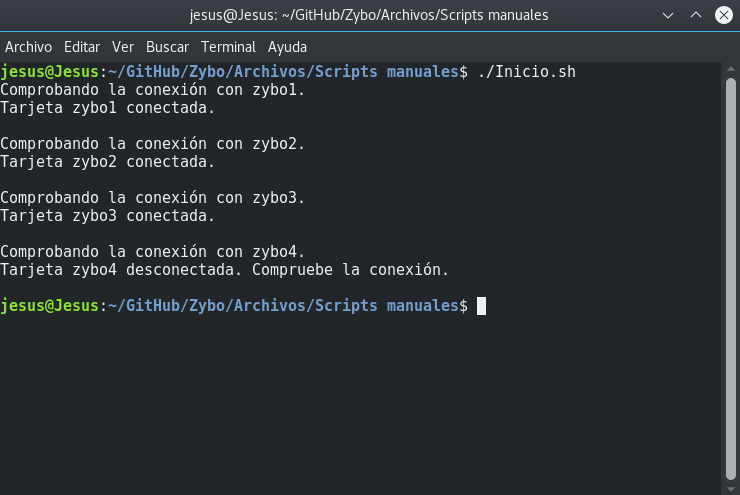
\includegraphics[scale=0.5]{Metodologia/Pruebas/Prueba_Inicio_sh.png}
	\caption{Prueba de \texttt{Inicio.sh}}
	\label{Prueba de Inicio.sh}
\end{figure}

\subsection{Software}
%\textcolor{red}{Prueba de funcionamiento de la recolección de datos: Una prueba de todo funcionando.}
Para realizar las pruebas de funcionamiento, basta con alimentar los nodos participantes en la cadena. En ese momento se ejecuta automáticamente los scripts descritos en el \hyperlink{Scripts}{Apéndice B}. 

Para el correcto funcionamiento de estos scripts, se requiere que el monitor central disponga del fichero inicial de datos creado por el usuario y que dicho usuario lo envíe al primer nodo de la red.

Hecho esto, sucede lo siguiente:
\begin{enumerate}
	\item Envío del fichero inicial a la primera tarjeta: Esto lo haremos gracias a la herramienta \texttt{sshpass} de Linux con la siguiente orden:
	\begin{center}
		\texttt{sshpass -p zyboX scp -o StrictHostKeyChecking=no archivoLocal zyboX@zyboX:/home/zyboX/ficheros/recibir}
	\end{center}
	Este proceso (Figura \ref{Fichero inicial en el ordenador central y envío al primer nodo}) lo podemos ver más detalladamente en el \hyperlink{EnvioRecepcionFicheros}{Apéndce A.4}.
	\begin{figure}[h]
		\centering
		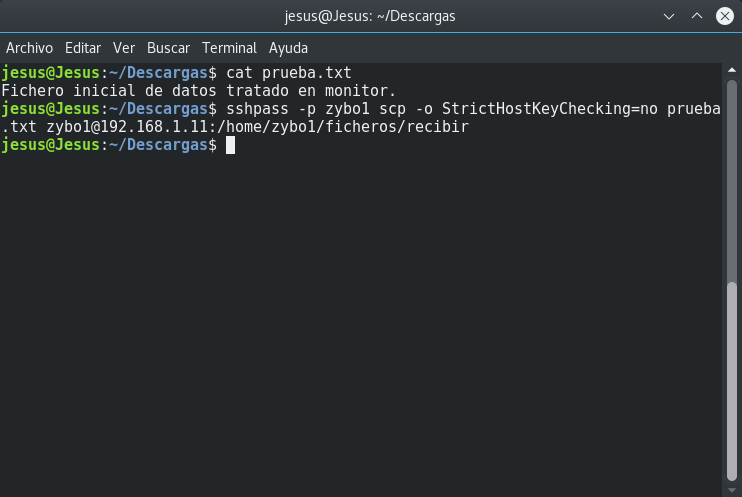
\includegraphics[scale=0.5]{Metodologia/Pruebas/Fichero_inicial_en_PC.png}
		\caption{Fichero inicial en el ordenador central y envío al primer nodo}
		\label{Fichero inicial en el ordenador central y envío al primer nodo}
	\end{figure}
\newpage
	\item Recepción del fichero en las tarjetas: Será el script \hyperlink{ScriptRecibiendo}{\texttt{Recibiendo.sh}} el encargado de comprobar la llegada del fichero y actuar en consecuencia cambiándolo de directorio.

	\item Modificación del fichero: El script \hyperlink{ScriptCristian}{\texttt{Cristian.sh}} será el encargado de abrir el fichero, modificarlo en cada una de las tarjetas y dejarlo preparado para su envío al siguiente nodo de la red. Para comprobar que los resultados de este script son correctos, podemos usar los comandos que vemos en la Figura \ref{Estado del fichero después de su modificación en Zybo1}.
	\begin{figure}[h]
		\centering
		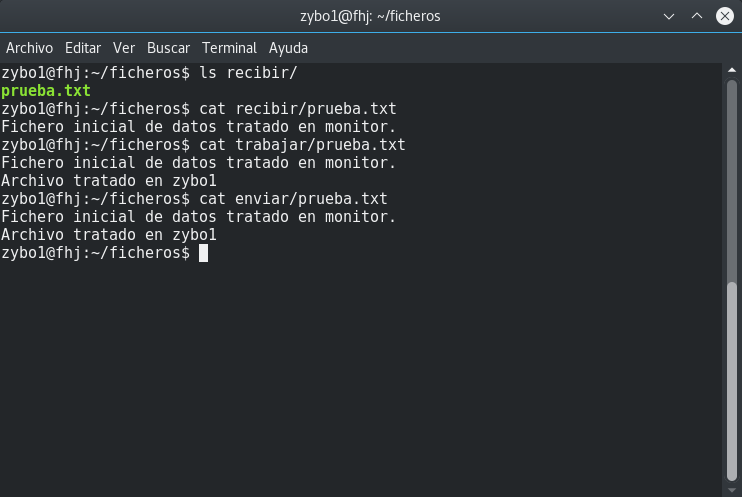
\includegraphics[scale=0.5]{Metodologia/Pruebas/Fichero_en_Zybo1.png}
		\caption{Estado del fichero después de su modificación en Zybo1}
		\label{Estado del fichero después de su modificación en Zybo1}
	\end{figure}
\newpage
	\item Envío del fichero hacia el siguiente nodo: Podemos distinguir dos tipos de envío del mismo fichero. Ambos llevados a cabo por el script \hyperlink{ScriptEnviando}{Enviando.sh}:
	\begin{enumerate}
		\item Tarjeta-Tarjeta: Esta opción se dará cuando la tarjeta actual detecte que la siguiente tarjeta está conectada.
		\item Tarjeta-Ordenador: Esta opción se dará cuando la tarjeta no detecte a la siguiente tarjeta. Entonces, enviará el fichero de datos, de vuelta al ordenador central.
	\end{enumerate}

\newpage
	\item Recepción del fichero en el ordenador central: El fichero final de datos, será recibido en el directorio\\ \texttt{/home/jesus/Vídeos} del ordenador central y contendrá los datos añadidos por todos los nodos de la red.
	\begin{figure}[h]
		\centering
		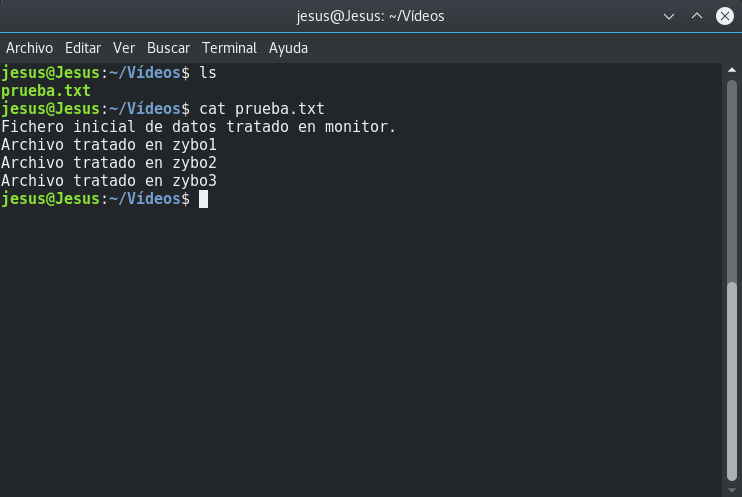
\includegraphics[scale=0.5]{Metodologia/Pruebas/Fichero_final_en_PC.png}
		\caption{Fichero final en el ordenador central}
		\label{Fichero final en el ordenador central}
	\end{figure}

\end{enumerate}